\graphicspath{{chapters/4_implementación/figures}}

\chapter{Implementación}\label{chap:implementation}

La primera decisión importante en el proceso de desarrollo fue implementar el algoritmo en la GPU.
La principal razón para esto es el alto grado de paralelismo que la misma ofrece.
A su vez, el ducto de rasterización, ampliamente implementado y optimizado en las GPUs, puede ser utilizado, aprovechando así algoritmos y cálculos optimizados a la hora de generar una imagen.

La programación en GPU precisa un lenguaje para la \textbf{CPU}, una \textbf{API de gráficos} y un lenguaje de \textbf{sombreado}.
El lenguaje de CPU es el que realiza y coordina las llamadas a funcionalidades de la GPU.
La API de gráficos es la que provee la interfaz que utiliza el lenguaje de CPU para comunicarse con la GPU.
La misma es una especificación que los fabricantes de las tarjetas de video deben implementar si deciden soportarla.
El lenguaje de sombreado es el que se utiliza para escribir los \textit{shaders}, programas que ejecutan directo en la GPU y hacen uso del paralelismo de la misma.

Como lenguaje de CPU se eligió \textbf{Rust}, un lenguaje de sistemas moderno multiparadigma.
Fue escogido debido a su gran comunidad, su amplia documentación y su poderoso manejador de paquetes \textit{cargo}.  
Se caracteriza por ser eficiente, al permitir un acceso a primitivas de bajo nivel, pero manteniendo una buena experiencia de desarrollo, debido a las abstracciones de costo cero que provee.
Otra característica a mencionar es la seguridad de memoria que impide comportamientos indefinidos en tiempo de ejecución como punteros nulos en situaciones que se espera un valor, o accesos a espacios de memoria no inicializados o liberados.

También se consideró el lenguaje C++ para CPU, dado que es el lenguaje más popular para aplicaciones gráficas.  
Si bien ambos lenguajes presentan una eficiencia similar, el factor que más pesó en la decisión fue la presencia de un manejador de paquetes en Rust.
El mismo permitió instalar varias dependencias más rápido y cambiarlas a lo largo del ciclo de desarrollo cuando fue necesario.
Dada la implementación en la GPU, la eficiencia y el manejo de memoria fue secundario. 

Como API de gráficos se eligió \textbf{OpenGL}, junto con el lenguaje de sombreado \textbf{GLSL}, el más usado para OpenGL, aunque soporte otros lenguajes.
También fueron consideradas CUDA y Vulkan, pero se terminó por escoger OpenGL debido a la facilidad de desarrollo, el conocimiento previo del equipo y la facilidad de trabajo con \textit{compute shaders}.
Si bien Vulkan es una API más moderna, es conocida por ser más compleja que OpenGL y el equipo del trabajo no contaba con la suficiente experiencia para utilizarlo adecuadamente.
CUDA suele usarse para cómputo de propósito general en la GPU, sin embargo, no posee ducto de rasterización, el cual fue ampliamente utilizado.
Por lo tanto, se optó por utilizar los \textit{compute shaders} de OpenGL para el cómputo de propósito general necesario.

El desarrolló se realizó en el sistema operativo \textbf{Linux} debido a los ambientes de desarrollo utilizados.
De igual manera, tanto Rust como OpenGL son multiplataforma, con lo que la aplicación es fácilmente portable a otros sistemas operativos.

La arquitectura de la aplicación consta de tres paquetes: \textit{CLI}, \textit{Core} y \textit{Engine}.
\textit{Engine} contiene todas las abstracciones sobre OpenGL utilizadas, provee tipos como \textit{Transform}, \textit{Light}, \textit{Camera}, comunes en aplicaciones interactivas, que permiten manipular objetos en el espacio 3D.
\textit{Core} contiene todas las etapas y programas del algoritmo que han sido mencionados: voxelización, construcción del \textit{octree}, filtrado, actualización y el trazado de conos en sí.
El paquete \textit{CLI} (\textit{Command-Line Interface}, interfaz por línea de comandos) es el punto de entrada de la aplicación, procesa los argumentos pasados por línea de comandos y archivos de configuración y utiliza las funcionalidades expuestas por \textit{engine} y \textit{core} para crear un ambiente 3D y ejecutar el algoritmo.
La arquitectura se muestra en la Figura \ref{fig:overall_architecture}.

\begin{figure}
    \centering
    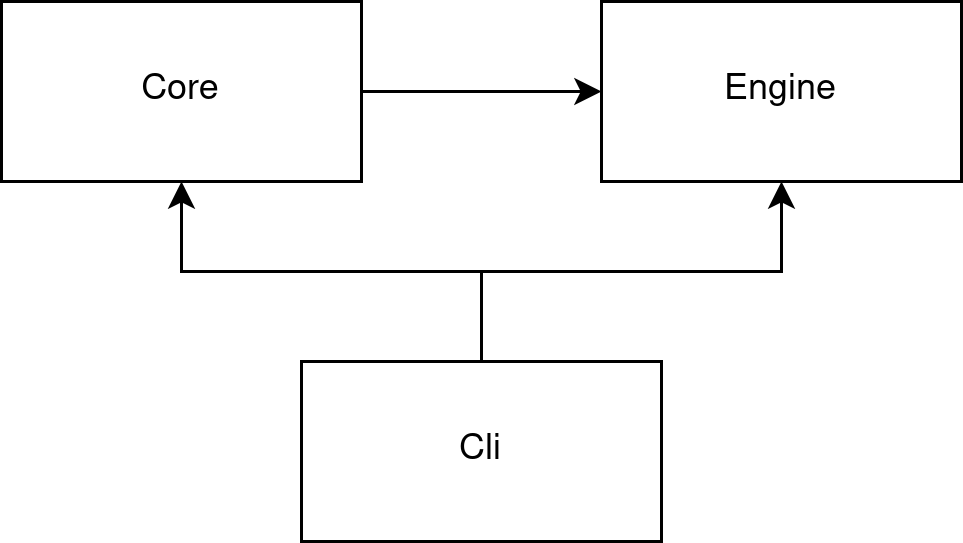
\includegraphics[width=.5\textwidth]{arquitectura_vct.png}
    \caption{Arquitectura alto nivel de la aplicación.}
    \label{fig:overall_architecture}
\end{figure}

En las siguientes secciones se verán más a detalle cada uno de estos paquetes.

\section{\textit{Engine}}

\begin{figure}[ht]
    \centering
    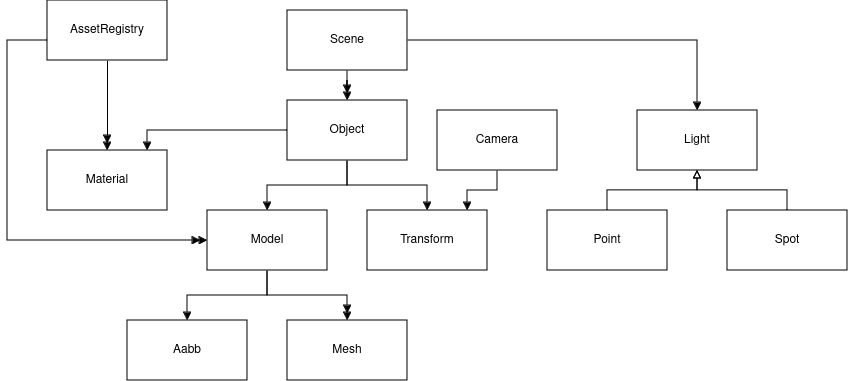
\includegraphics[width=\textwidth]{diagram_engine.png}
    \caption{Arquitectura de \textit{Engine}.}
    \label{fig:engine_architecture}
\end{figure}

\textit{Engine} es el paquete en el que se implementaron las abstracciones usuales al trabajar con API de gráficos, que son utilizadas por el resto de la aplicación.
Se pueden ver con sus relaciones en la Figura \ref{fig:engine_architecture}.

La abstracción principal es la escena (\textit{Scene}).
Una escena consta de una luz (\textit{Light}) y de muchos objetos (\textit{Object}).
Es la representación del mundo tridimensional en el que se encuentra todo lo visible de la aplicación.

Cada objeto de la escena tiene un material (\textit{Material}), un modelo (\textit{Model}) y un \textit{Transform}.

\textit{Transform} es un tipo que contiene la posición, rotación y escala de un objeto en la escena.
Esto simplifica el lidiar con matrices de traslación, rotación y escala a lo largo de todo el programa.

Tanto los modelos como los materiales son cargados una vez al inicio de la aplicación en el \textit{AssetRegistry} para no duplicarlos en caso de que sean utilizados por más de un objeto.
Los objetos solo necesitan almacenar referencias a estos.

Se representan los modelos como mallas poligonales, distinto al trazado de rayos en el que se usan ecuaciones geométricas.
Para cargar estos modelos, se utilizó la librería \textit{tobj} \cite{tobj-crate}, que permite cargar archivos con extensión \textit{obj}.
Cada \textit{Model} contiene muchos \textit{Mesh} y tiene un \textit{Aabb}, un Axis-Aligned Bounding Box, que se calcula a partir de cada uno de los vértices del mismo.
Este volumen acotante se calcula en el momento que se carga el modelo y se expone para ser utilizado por el resto de la aplicación.

\textit{Camera} provee el punto de vista, la dirección de vista, la dirección hacia arriba, la ventana de vista, entre otros, del que se renderiza toda la escena.
Se soportan tanto cámaras en perspectiva como ortogonales.

Para las luces, se soportan tanto luces direccionales como puntuales.
Estas luces tienen toda la lógica necesaria para que luego \textit{core} realice la inyección de fotones.

La estructura de árbol, los bricks, y todas las estructuras auxiliares, se almacenan en la memoria de la GPU.
Para esto, se ofrecen abstracciones sobre los distintos tipos de memorias y texturas de la GPU.
\textit{TextureBuffer}, \textit{Texture2D} y \textit{Texture3D} son ejemplos de estas, que manejan memoria lineal, bidimensional y tridimensional respectivamente.
Se provee la abstracción \textit{Shader} para interactuar con la GPU mediante programas escritos en GLSL.

Finalmente, se exponen las primitivas necesarias para crear una interfaz de usuario.
Luego, estas son usadas por \textit{core} para modificar parámetros del algoritmo.

\section{Core}

\begin{figure}[ht]
    \centering
    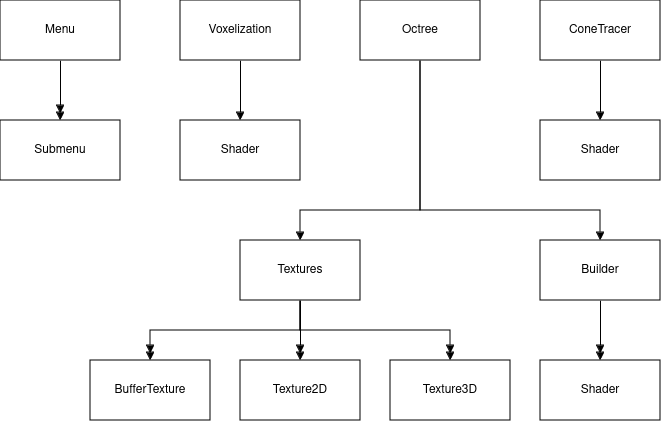
\includegraphics[width=\textwidth]{diagram_core.png}
    \caption{Arquitectura de \textit{Core}.}
    \label{fig:core_architecture}
\end{figure}

\textit{Core} es el corazón de la implementación, donde se implementa el algoritmo.
Contiene la lógica de la voxelización, toda la implementación del \textit{octree}, el trazado de conos y un menú para poder ajustar parámetros en tiempo de ejecución.
Debido a que el algoritmo está implementado en la GPU, este paquete hace mucho uso de los \textit{Shaders}.
Sus componentes se pueden ver en la Figura \ref{fig:core_architecture}.

\subsection{Etapas del algoritmo}

En la Figura \ref{fig:core_architecture} se pueden ver los componentes encargados de cada etapa del algoritmo.

La voxelización tiene su propio módulo que hace uso del ducto de rasterización como se vio en \ref{sec:voxelization}.
Para voxelizar la escena, está primero debe ser normalizada usando el \textit{Aabb} expuesto por \textit{Engine}.
Se crea un \textit{Aabb} para la escena, y se le aplican transformaciones de escalado y translación de manera que sea lo más grande posible, pero quede incluida dentro de la grilla de vóxeles.
Las mismas transformaciones luego se aplican a los modelos al momento de voxelizar, asegurando así que todo objeto quede dentro de la grilla, y que se mantengan las proporciones.

La abstracción de \textit{Octree} realiza tanto construcción como el filtrado de los valores de la escena a lo largo de él.
Guarda referencias a todas las texturas utilizadas y a todos los \textit{Shaders} que operan sobre esas texturas.
También guarda una referencia a la lista de vóxeles generada por el módulo anterior.

El \textit{ConeTracer} reúne todos los conceptos anteriores e implementa el algoritmo de trazado de conos en el ducto de rasterizado, donde se genera la imagen final.

\subsection{Representación del \textit{octree}}

La estructura del \textit{octree}, cada nodo y sus hijos, se representa en la GPU con una textura lineal.
Esta textura se llama \textit{node pool}.
Cada téxel (elemento de textura) de esta textura es un puntero a otro nodo.
Se toma la convención de que cada grupo de 8 téxeles es un nodo, donde cada téxel es un puntero al hijo correspondiente.
Los primeros 4 téxeles representan los hijos con valor de $z = 0$ mientras que los últimos 4 representan los que tienen valor de $z = 1$.
De manera similar de cada grupo de 4, los primeros 2 son los hijos con valor de $y = 0$ menor y los otros dos $y = 1$.
Por último de cada uno de los 4 grupos de 2, el primer téxel representa al hijo con coordenada $x = 0$ y el último con coordenada $x = 1$.
Si un téxel tiene el valor $0$, entonces ese hijo del nodo representa espacio vacio, y ese nodo no será guardado en la \textit{node pool}.
Si un téxel tiene un valor $n \not = 0$, entonces en la posición de memoria $n * 8$ comienza ese nodo, que termina en la posición de memoria $x * 8 + 7$.

\begin{figure}[h!]
    \centering
    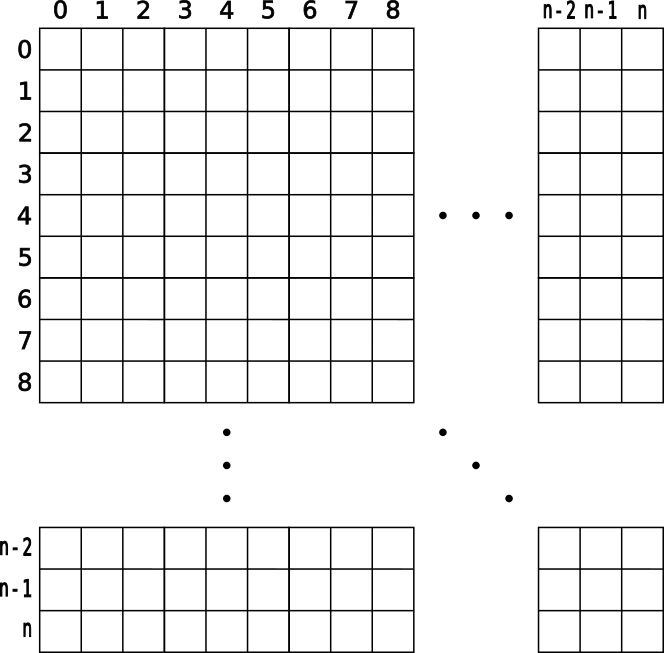
\includegraphics[width=\textwidth]{bricks-memory-big-borders.png}
    \caption{Ejemplo de \textit{brick pool} (en 2D), con índices de memoria. El verdadero es 3D.}
    \label{fig:brick_pool_example}
\end{figure}

Para representar los \textit{bricks}, se usa una gran textura 3D, llamada la \textit{brick pool}.
Cada brick es una sección de $3^3$ téxeles de esta textura 3D.
En cada uno de estos téxeles se almacenan valores de la escena, por ejemplo color.
Para otros valores que deben ser almacenados, como la irradiancia, se crea otra \textit{brick pool}.
Cada téxel dentro de un brick se llama vóxel, porque además de ser un píxel de textura, también es un píxel de volumen, a los efectos de la aplicación.
En la Figura \ref{fig:brick_pool_example} se muestra una \textit{brick pool}, con una textura 2D para facilitar la visualización, donde cada téxel está identificado por sus coordenadas $x$ e $y$ (y $z$ en su versión 3D).

\begin{figure}[h!]
    \centering
    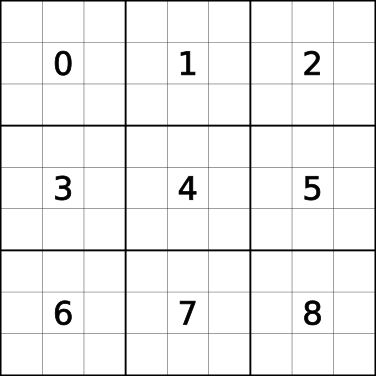
\includegraphics[width=0.5\textwidth]{indexed-bricks.png}
    \caption{Ejemplo de bricks, cada uno con un identificador único que se asocia a un nodo.}
    \label{fig:indexed_bricks}
\end{figure}

\begin{figure}[h!]
    \centering
    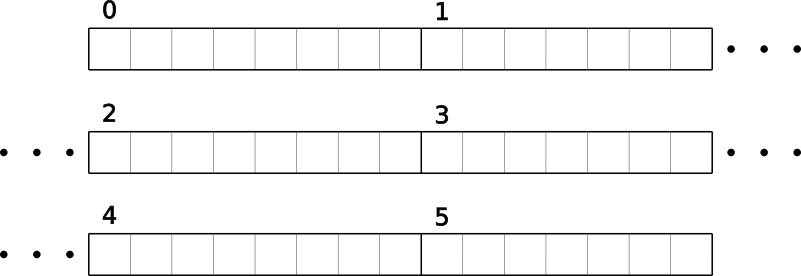
\includegraphics[width=\textwidth]{indexed-nodes.png}
    \caption{Ejemplo de nodos, cada uno con un identificador único.}
    \label{fig:indexed_nodes}
\end{figure}

Cada nodo tiene asociado un brick, ambos identificados de forma única por un mismo índice, como se puede ver en las figuras \ref{fig:indexed_bricks} y \ref{fig:indexed_nodes} respectivamente.
Dado que los bricks existen en una textura 3D, la manera de localizarlo en memoria es con un vector en $\mathbb{N}^3$.
Para esto, si se quiere encontrar el brick correspondiente a un nodo dado su identificador, dado que nodo y brick comparten un mismo identificador en $\mathbb{N}$, se usa una función que convierte el índice del nodo en un vector en $\mathbb{N}^3$.
El vector de $\mathbb{N}^3$ $(n, m, s)$ es el índice del primer vóxel del brick buscado.
El resto del \textit{brick} se encuentra en las posiciones desde $(n, m, s)$ hasta $(n + 2, m + 2, s + 2)$.

\begin{figure}[h!]
    \centering
    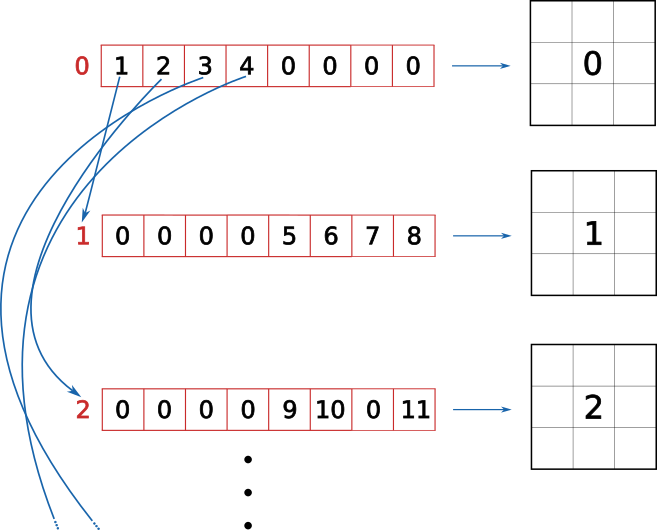
\includegraphics[width=\textwidth]{nodes-n-bricks.png}
    \caption{Ejemplo node pool y brick pool.}
    \label{fig:nodes_n_bricks}
\end{figure}

En la Figura \ref{fig:nodes_n_bricks} se muestra un ejemplo de nodos, con sus bricks asociados.
Además, cada nodo contiene $8$ téxeles, los cuales representan los hijos del nodo, donde el valor de cada téxel es el identificador de un nodo.

Ya que el árbol es disperso se necesita un valor que represente que un hijo no contiene geometría, que representa espacio vacío.
Se usa el valor 0.
Cada téxel apunta a un nodo mediante su índice en la \textit{node pool}.
En la figura se muestran estos índices dentro de cada téxel.

Se usa el índice del nodo para identificar su \textit{brick}, que es parte de una textura 3D.
Cada brick se muestra al costado de su nodo asociado, con sus coordenadas dentro de la textura en el margen derecho.
Cada téxel individual de un brick tiene sus propias coordenadas, como es el caso con los téxeles individuales de la \textit{node pool}.

Propiedades de la escena, ya sea color o irradiancia, se almacenan en los \textit{bricks}.
Existe una función que lleva posiciones dentro del nodo, que representa una sección de la escena, a posiciones dentro de su brick asociado.
En la Figura \ref{fig:node_and_brick} se vé porque es necesario, las esquinas del nodo se mapean a los centros de los vóxeles del brick.
A la hora de tomar una muestra de una propiedad en un punto de la escena, se úbica el nodo correspondiente, se aplica la función y se toma el valor de la propiedad en el \textit{brick}.
Si el punto no es el centro de uno de los vóxeles del brick, se debe interpolar el valor utilizando los vóxeles adyacentes.
Almacenar los bricks en una textura 3D en lugar de en una textura lineal trae beneficios de rendimiento, ya que las GPU proveen interpolación trilineal acelerada por hardware, lo que elimina la necesidad de implementarla, y se obtiene mayor rendimiento.

% TODO: Agregar una referencia acá
\subsection{Renderizado diferido}\label{sec:deferred-rendering}

Para renderizar la escena, se utiliza el renderizado diferido.

A la hora de renderizar una escena, hay dos grandes modelos que se pueden utilizar: el clásico, conocido como \textit{forward rendering} y una opción alternativa conocida como renderizado diferido.

En el primero, se procesan todos los vértices en el programa.
Cada uno pasa por cada etapa del ducto gráfico y aporta a la imagen final a menos que sea desechado por una prueba de profundidad.
Cuando un píxel genera varios fragmentos, y se deben correr calculos pesados por fragmento, se puede estar realizando trabajo innecesario, debido a que, en el espacio 3D de la escena, pueden estar a distinta profundidad y solo el más cercano es el que se debe procesar.
Dados dos fragmentos que podrían darle color a un mismo píxel, una prueba de profundidad descartará al que se encuentre detrás del otro, a menos que presente opacidad menor a 1.

En el renderizado diferido, se procesan todos los vértices del programa, pero se saltean calculos pesados en el \textit{fragment shader}.
Se guarda toda la información necesaria para etapas posteriores en texturas llamadas \textit{geometry buffers}, datos como posicion, normal, color y cualquier otro dato relevante de la geometria a la hora de realizar calculos pesados de sombreado.
% TODO: Hablar del volumen de vista?
Se saltean los cálculos para objetos fuera del campo de visión y detrás de otros objetos.

El \textit{forward rendering} es conceptualmente más sencillo y más fácil de implementar.
En escenas con pocos objetos y fuentes de luz, o con calculos simples de iluminacion, la complejidad extra del renderizado diferido no suele estar justificada dado que el aumento de rendimiento es despreciable.
A su vez, el \textit{forward rendering} soporta mejor la opacidad.
Sin embargo, a medida que la complejidad de la escena y los metodos de sombreado aumenta, el renderizado diferido se vuelve cada vez una mejor opción para aumentar el rendimiento.
También, el renderizado diferido facilita ciertas técnicas de postprocesamiento de la imagen, como \textit{bloom}, \textit{HDR} (\textit{High Dynamic Range}), corrección gamma, y normalización, entre otras.

\subsection{Menú}

A lo largo de la implementación, fue necesario depurar varios errores y correr pruebas.
Para esto, fue muy útil contar con una interfaz gráfica o menú para seleccionar varias opciones y poder ver valores de la GPU en tiempo real.
Se desarrolló este menú utilizando un paquete del ecosistema de Rust llamado \textit{Egui} \cite{egui}.

\textit{Egui} permite rápidamente crear una interfaz gráfica basada en ventanas que se renderiza junto con la aplicación en cada frame.
Es muy sencillo conectar valores del código a etiquetas en el menú y botónes en el menú a acciones.

El menú de la aplicación cuenta con varias ventanas, o submenúes, para ver valores, ajustar parámetros, y renderizar distintas imágenes.
Uno de submenúes para depurar muestra todos los nodos de la \textit{node pool}, permite buscarlos por índice y coordenadas, y visualizarlos en el espacio.

Esta se puede ver en la Figura \ref{fig:node-positions-menu}.
En el menú se muestran todos los nodos con su índice en el buffer y sus coordenadas dentro de la escena, entre $0$ y la cantidad de vóxeles por dimensión, $512$ o $1024$.
Al apretar cualquier nodo, se muestra en la escena un cubo delimitando la región de la escena representada por ese nodo.
Se pueden mostrar muchos nodos a la vez.

\begin{figure}
    \centering
    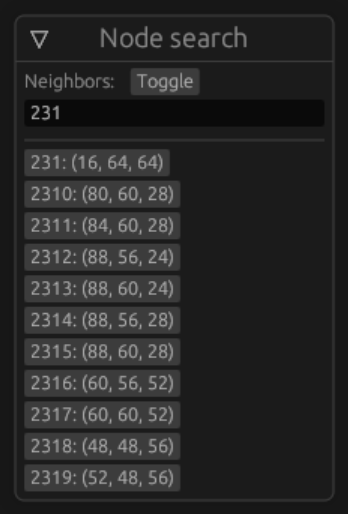
\includegraphics[width=.25\textwidth]{node-positions-menu.png}
    \caption{Menú de nodos.}
    \label{fig:node-positions-menu}
\end{figure}

También se usó la interfaz gráfica para reportar los FPS que fueron usados en el capítulo \ref{chap:experiments}.

\section{CLI}

\textit{CLI} (\textit{Command-Line Interface}, interfaz por línea de comandos), es el punto de entrada de la aplicación.
Consta de un archivo \textit{main} que inicializa el contexto de OpenGL, la ventana de la aplicación, y utiliza \textit{engine} y \textit{core} para crear la escena con iluminación global.
También procesa varios tipos de archivos de configuración, que serán explicados a continuación.
Todos estos tipos de archivos contienen información en formato RON, por \textit{Rusty Object Notation}, una notación similar a JSON, \textit{JavaScript Object Notation}, pero diseñada para Rust.

\subsection{Archivo de configuración}

Cada ejecución de la aplicación carga un archivo de configuración que se encarga de definir ciertos parámetros.
Estos son la cantidad de vóxeles que se utilizarán, $256$, $512$ o $1024$; las dimensiones de la pantalla, entre otros.
A partir de esto, se inicializan otras variables, como la cantidad de niveles del octree, que es definida por la cantidad de vóxeles utilizados.
Estos parámetros son utilizados a lo largo de toda la aplicación, por lo que se usó el patrón singleton, creando un tipo \textit{Config}, que es inicializado una vez por \textit{CLI} y luego utilizado en el resto de la aplicación.

\subsection{Archivos de escena}

Para poder fácilmente cargar distintos modelos y probar el algoritmo en ellos, se creó un formato de archivos de escena.

En estos archivos se definen la lista de objetos y luces de la escena.
También se especifican listas de recursos para que los objetos referencien, modelos y materiales.
Estos recursos son cargados primero y los objetos pueden reutilizarlos sin necesidad de copiarlos.

Utilizando estos archivos, se pueden definir muchas escenas distintas para probar la implementación.

\subsection{Archivos de valores predeterminados}

Para poder iterar más rápido, se crearon archivos de valores predeterminados.
Estos archivos contienen valores predeterminados de opciones que cambian con el transcurso de la ejecución.
Por ejemplo, la posición de la cámara, qué tipo de imagen se está renderizando, qué nodos están siendo visualizados.
Estos archivos también pueden guardarse a partir del menú.

Al iniciar el programa, se puede especificar un archivo de valores predeterminados, que altera el estado inicial de la escena.
Son muy útiles cuando se está investigando algo en específico o viendo una imagen desde un punto de vista particular.
Es posible guardar los valores utilizados, cambiar algo en el código, recompilar y observar cómo ese cambio afectó lo que se estaba observando.

\section{Limitaciones}

Al implementar el algoritmo, se pudieron observar algunas limitaciones inherentes al uso de vóxeles.

Debido a que el algoritmo simula únicamente un rebote de la luz, la luz indirecta debería estar presente únicamente en zonas cercanas a las iluminadas directamente.
Excepto que le llegue el reflejo de alguno otra superficie, no debería haber luz indirecta en las mismas zonas donde hay luz directa.
Sin embargo, existen situaciones en las que esto sucede, como por ejemplo en la de la Figura \ref{fig:indirect-grabs-direct}.
En esta, se puede observar que la zona iluminada directamente también presenta un fuerte componente luz indirecta.

La Figura \ref{fig:indirect-grabs-direct-diagram} muestra un diagrama para ayudar a explicar este fenómeno.
En la derecha de la imagen hay una pared roja, rodeada de espacio vacío.
A la izquierda de la pared se muestran vóxeles de tamaños cada vez mayores y color cada vez más transparente.
Al trazar un cono desde la pared para calcular la luz indirecta sobre la misma, este terminará muestreando varias veces el mismo color que la pared.
Al no recibir luz que reboto de ninguna otra superficie, se puede observar como la luz indirecta sobre la pared acaba incluyendo el rebote de luz de la pared misma, por lo que la luz directa termina afectando dos veces.

\begin{figure}[h]
    \begin{center}
    \begin{subfigure}{.49\textwidth}
        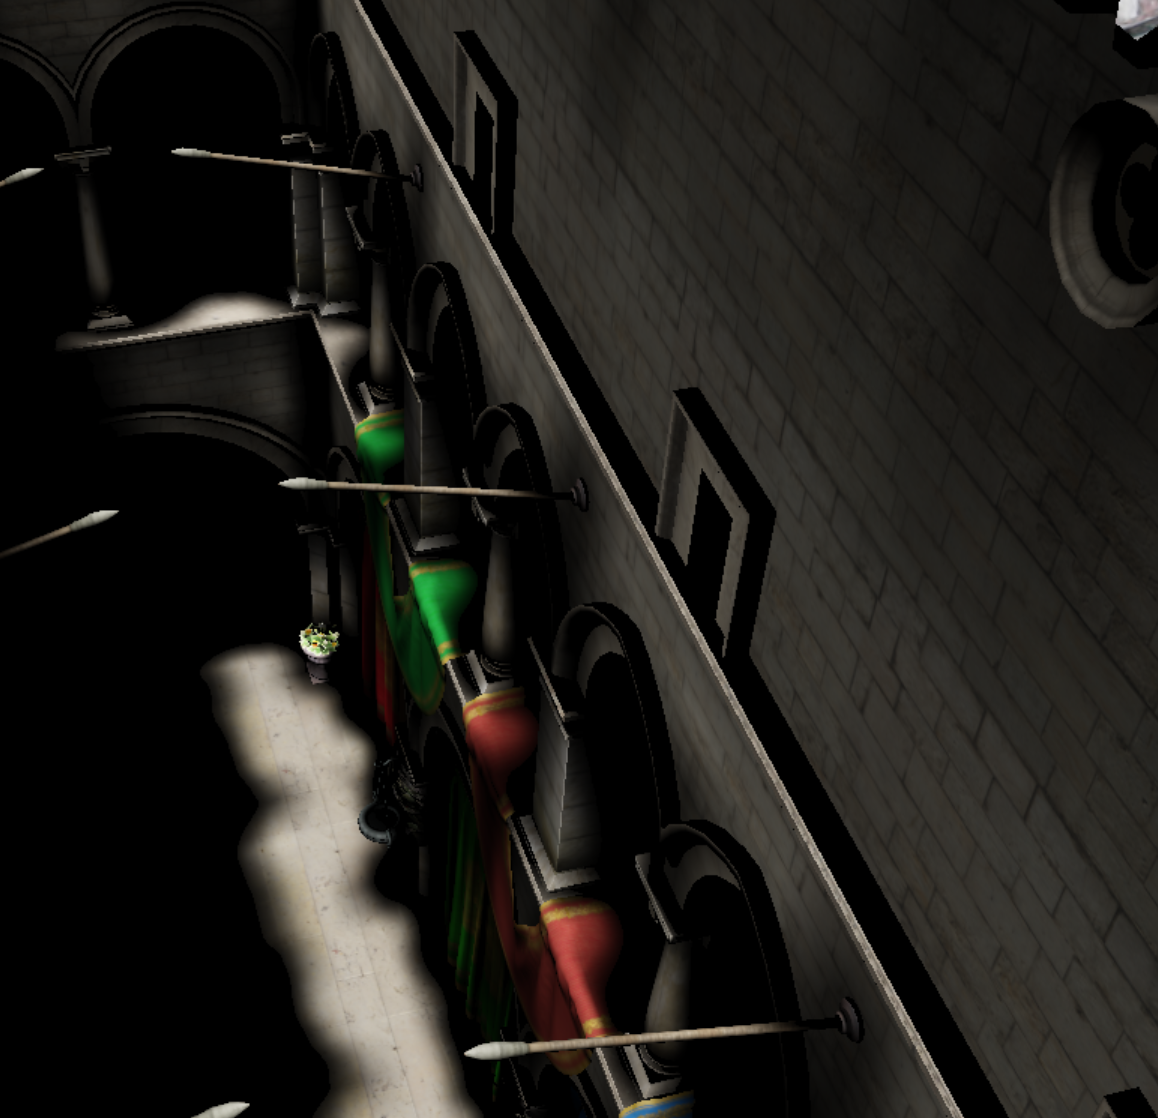
\includegraphics[width=\textwidth]{indirect-grabs-direct-1.png}
        \caption{Solo luz directa.}
    \end{subfigure}
    \begin{subfigure}{.49\textwidth}
        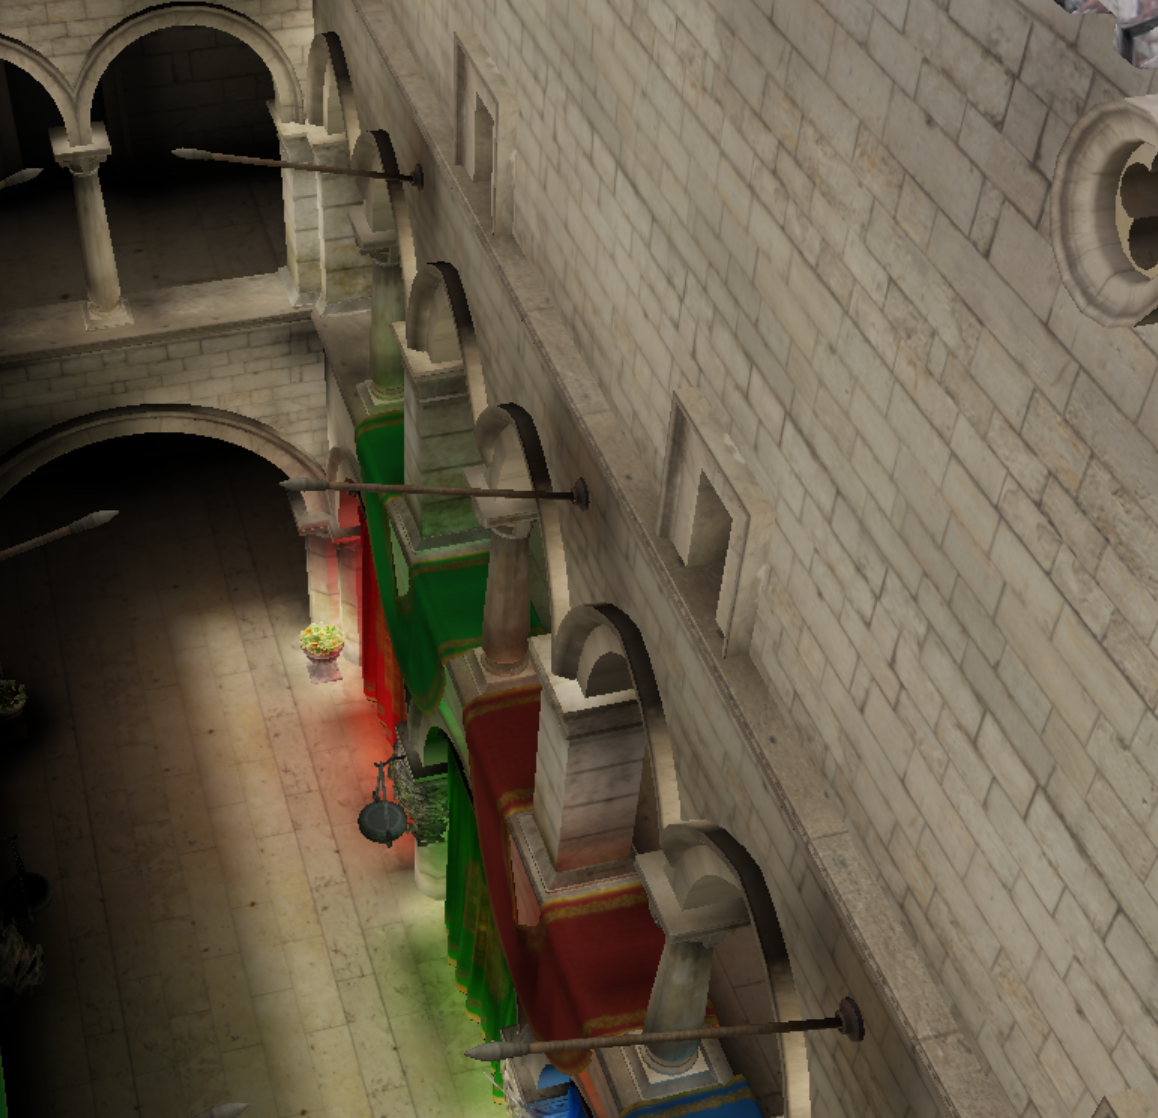
\includegraphics[width=\textwidth]{indirect-grabs-direct-2.png}
        \caption{Solo luz indirecta.}
    \end{subfigure}
    \caption{Luz indirecta incluye la directa.}
    \label{fig:indirect-grabs-direct}
    \end{center}
\end{figure}

\begin{figure}[h]
	\begin{center}
	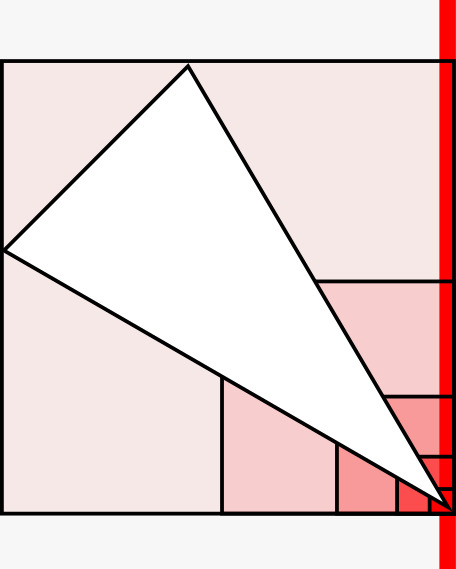
\includegraphics[width=0.5\textwidth]{indirect-grabs-direct-diagram.png}
	\caption{Cono muestreando el mismo color de la pared.}
	\label{fig:indirect-grabs-direct-diagram}
	\end{center}
\end{figure}

Otra limitación se observa en la Figura \ref{fig:indirect-behind-banner}, donde se muestra la presencia de luz indirecta detrás de un estandarte.
En un escenario real, la luz no debería rebotar detrás del estandarte, sino únicamente en el frente.
Dado que no se maneja refracción, luz ubicada al frente del estandarte no debería ser tomada por la pared atrás del mismo.
Sin embargo, esto ocurre porque la superficie del estandarte es muy delgada, y la unica capa de vóxeles que lo representan abarcan tanto el lado frontal como el posterior.
Este problema es resuelto agregando una mayor resolución, ya que esto genera dos capas de vóxeles para los estandartes, por lo que a la pared no le afecta la luz reflejada la cara frontal del estandarte.

\begin{figure}[h]
    \begin{center}
    \begin{subfigure}{.49\textwidth}
        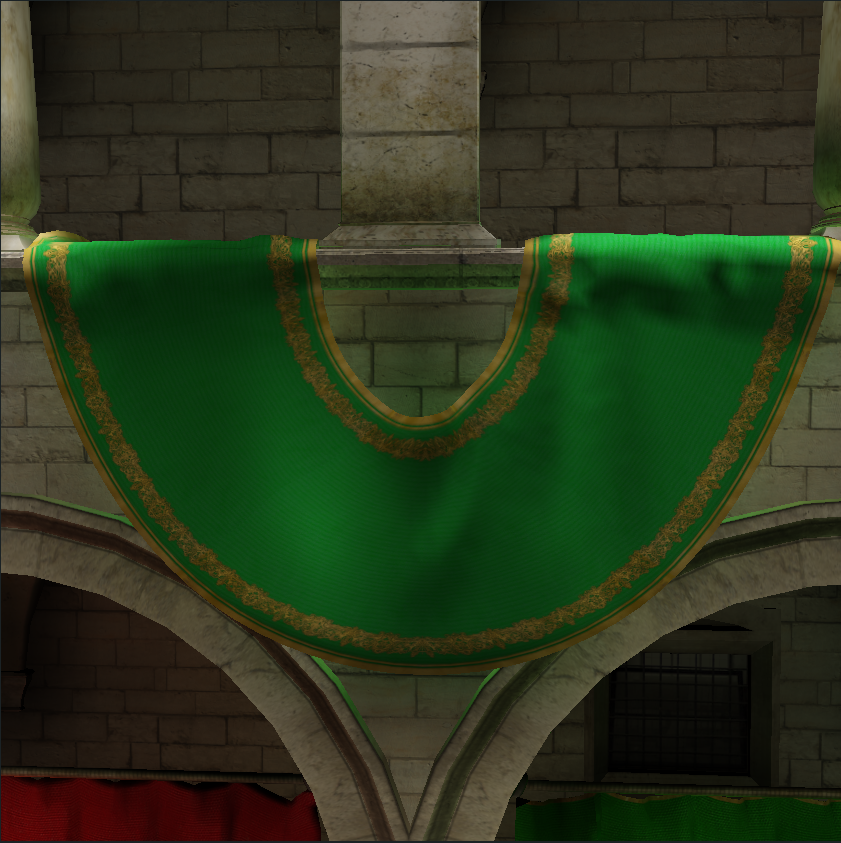
\includegraphics[width=\textwidth]{limitations-behind-banner-side.png}
        \caption{Luz indirecta detrás de un estandarte (costado).}
    \end{subfigure}
    \begin{subfigure}{.49\textwidth}
        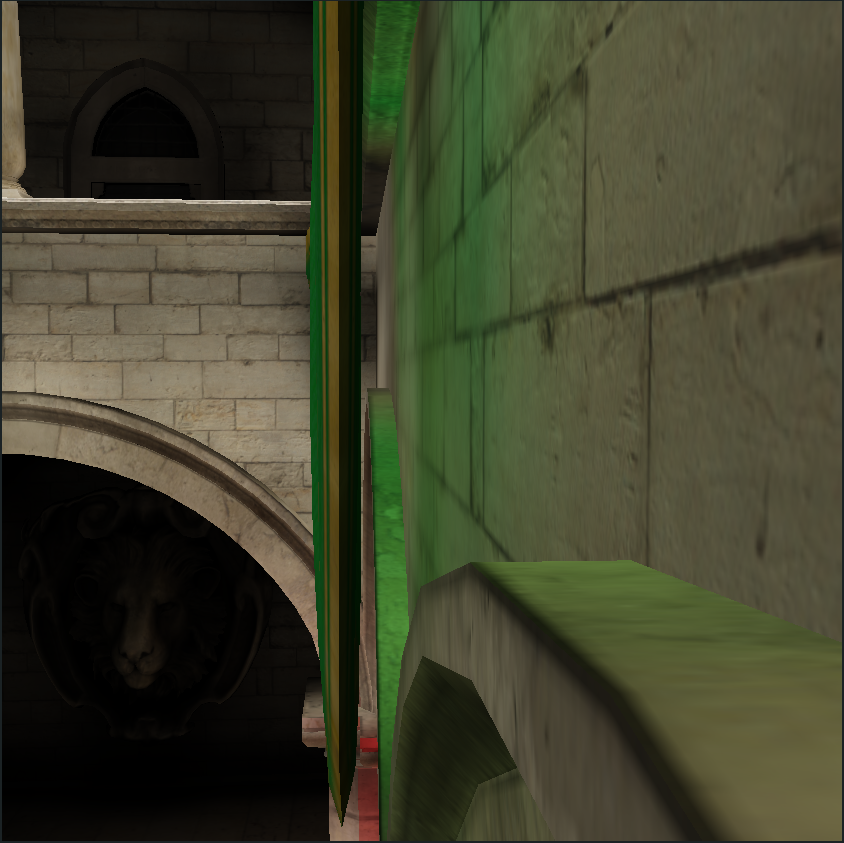
\includegraphics[width=\textwidth]{limitations-behind-banner-front.png}
        \caption{Luz indirecta detrás de un estandarte (frente).}
    \end{subfigure}
    \caption{Luz indirecta incluye la directa.}
	\label{fig:indirect-behind-banner}
    \end{center}
\end{figure}
